\pagebreak
\section{Travail réalisé}

\subsubsection{Cas pratique 1}
Tous les points exigés par la donnée ont été réalisés. Voici un aperçu des deux différentes vues du projet, la tableView et la vue pour ajouter/éditer une tâche :

\begin{figure}[H]
	\begin{center}
		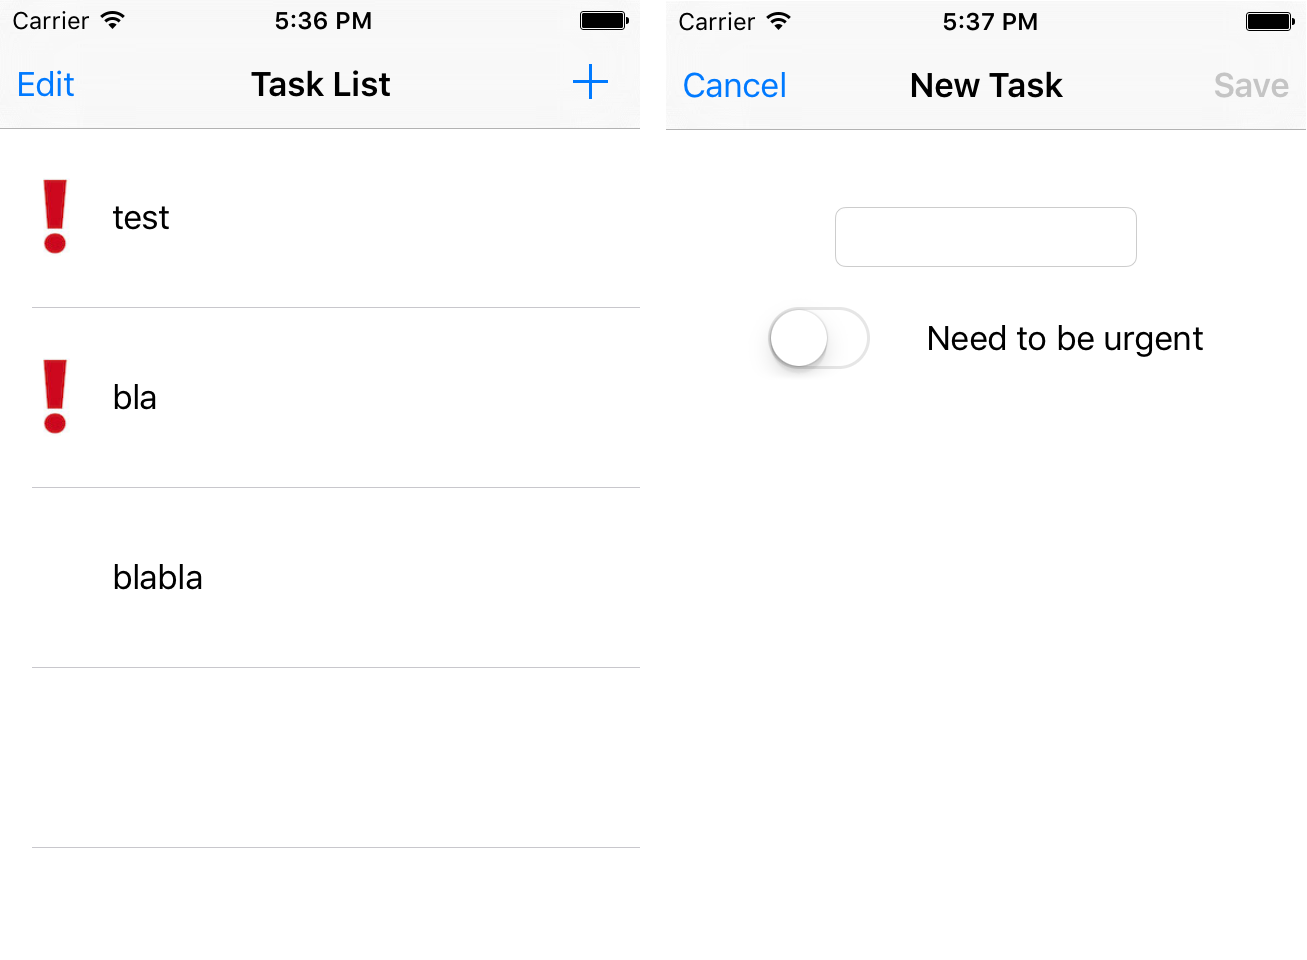
\includegraphics[width=14cm]{img/cas1_0.png}
		\caption{Vues de l'application réalisée}
		\label{vues}
	\end{center}
\end{figure}
\textbf{Source de l'image !:\\}
\url{http://static.guim.co.uk/sys-images/Guardian/Pix/pictures/2009/4/29/1240996556472/exclamation-001.jpg}\\\\

\textbf{Suppression d'une tâche:}\\
Pour supprimer une tâche de la liste, deux procédés sont possibles. On peut soit cliquer sur le bouton Edit, qui affiche un symbole "-" à côté de chaque tâche, soit directement faire un swipe sur la gauche de la tâche. Les deux méthodes affichent le bouton delete qui enlèvera l'entrée de la liste.\\
Avec les deux méthodes, le bouton Edit se transforme en Done pour terminer l'action.

\begin{figure}[H]
	\begin{center}
		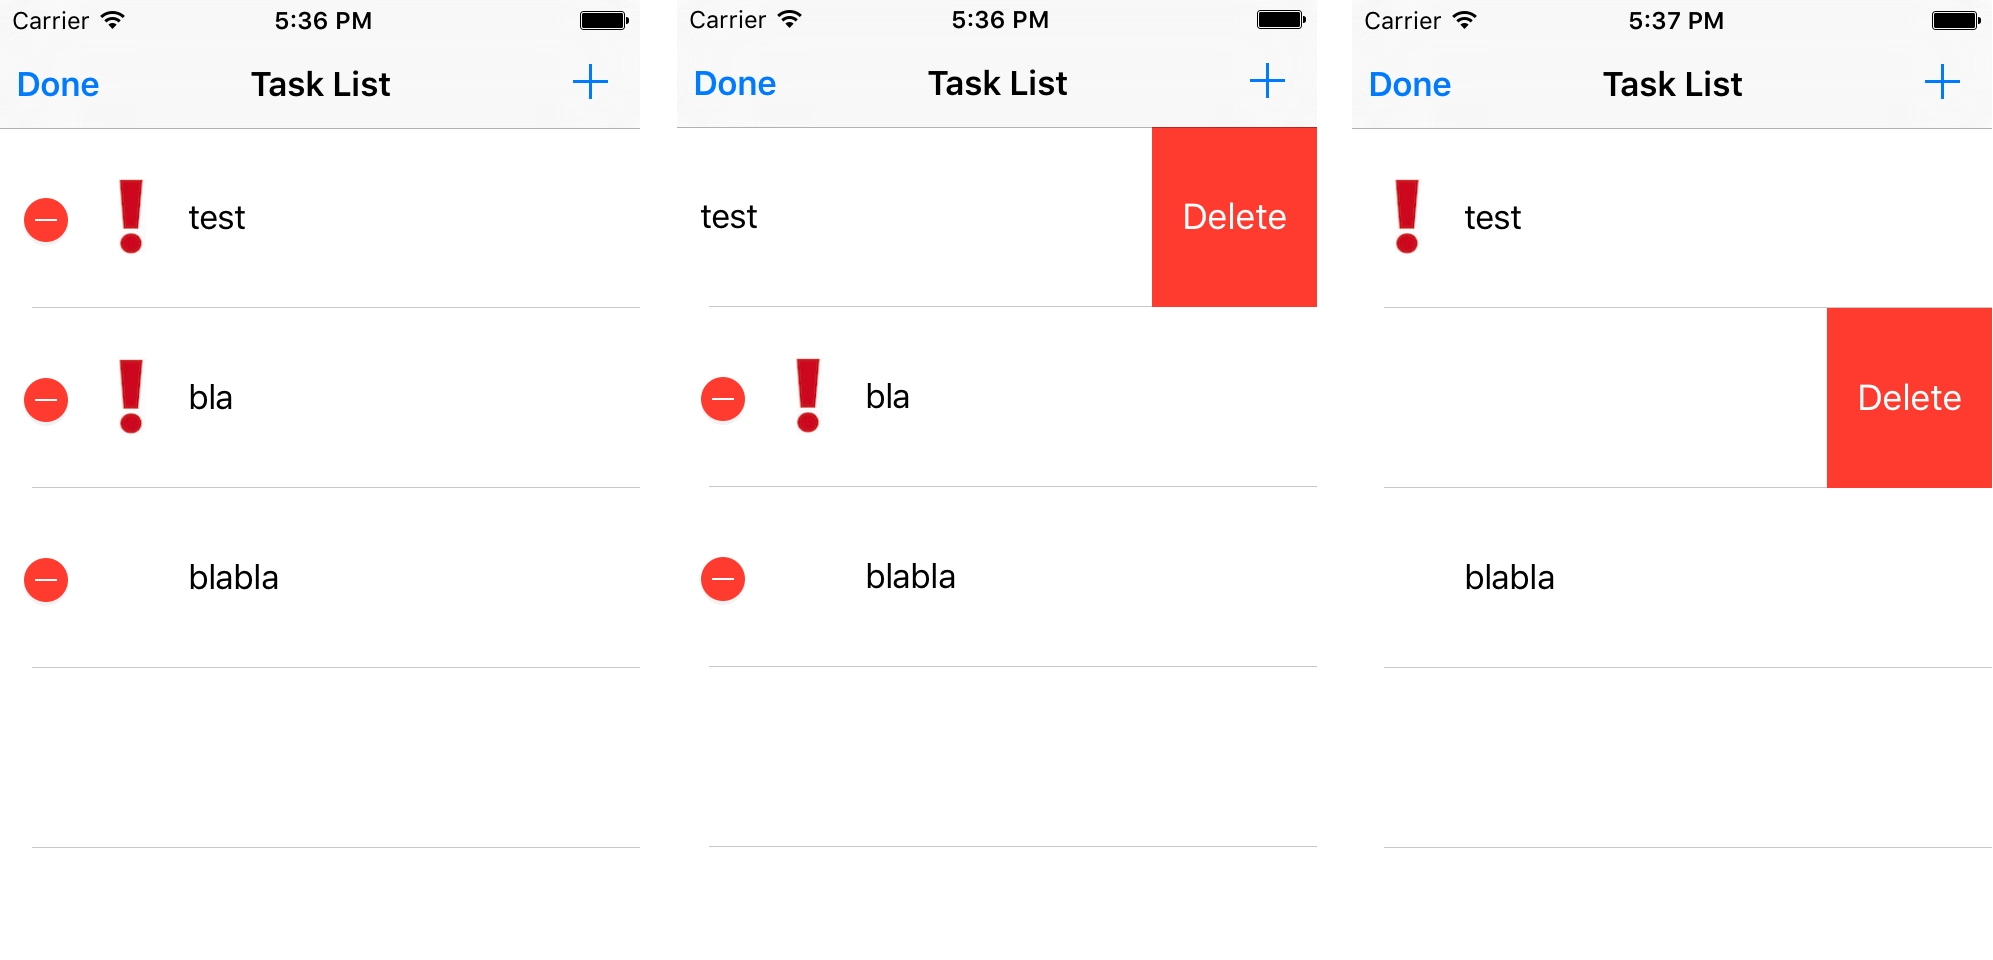
\includegraphics[width=16.5cm]{img/cas1_01.png}
		\caption{Edit method (left and middle) - swipe method (right)}
		\label{vues1}
	\end{center}
\end{figure}

\textbf{Edition/ Ajout d'une tâche:}\\
Quand on édite une tâche, ses informations sont reportées dans la nouvelle vue, alors que quand on en ajoute une, la nouvelle vue est vide. La liste est ensuite mise à jour.

\begin{figure}[H]
	\begin{center}
		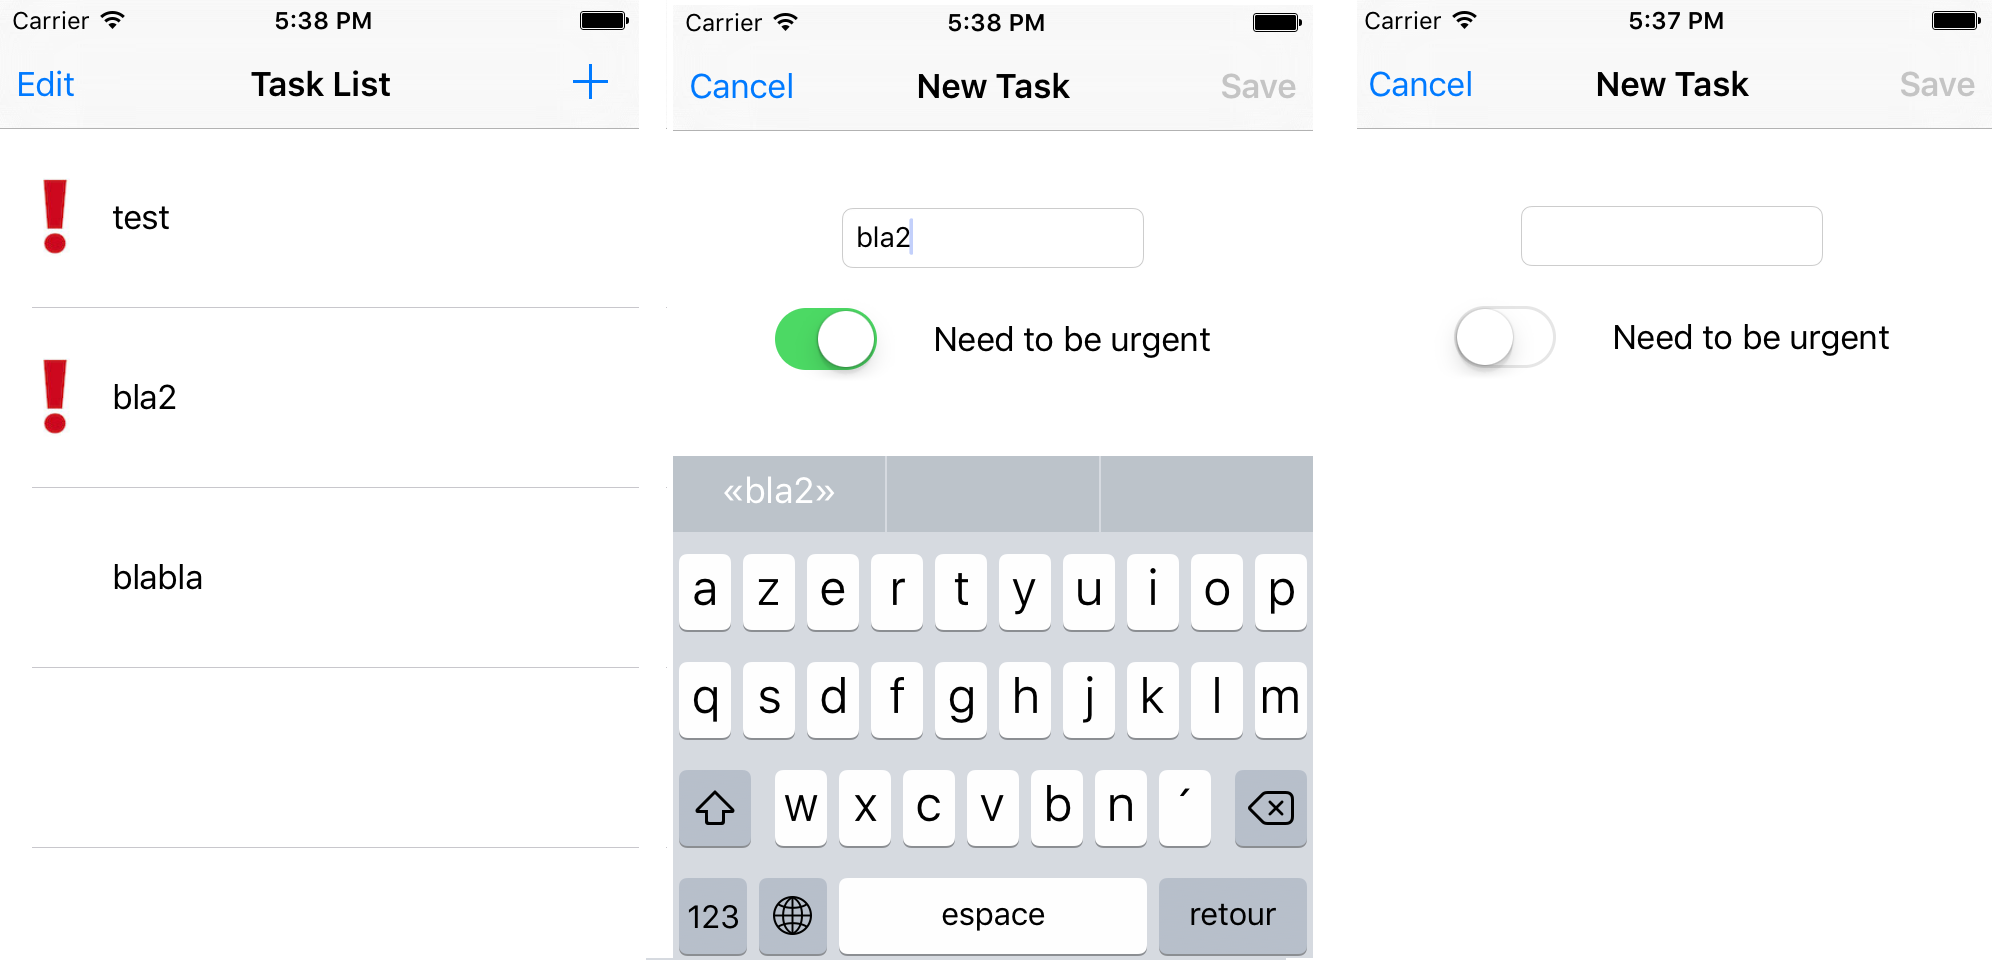
\includegraphics[width=16.5cm]{img/cas1_02.png}
		\caption{Edit task (left and middle) - Add task (right)}
		\label{vues2}
	\end{center}
\end{figure}

\textbf{Sauvegarde des tâches:}\\
Lorsque l'on relance l'application, les tâches que l'on a créées précédemment sont présentes.

\subsubsection{Cas pratique 2}
Tous les points exigés par la donnée ont été réalisés sauf la partie concernant la musique. Voici un aperçu des différentes vues du projet:
\begin{figure}[H]
	\begin{center}
		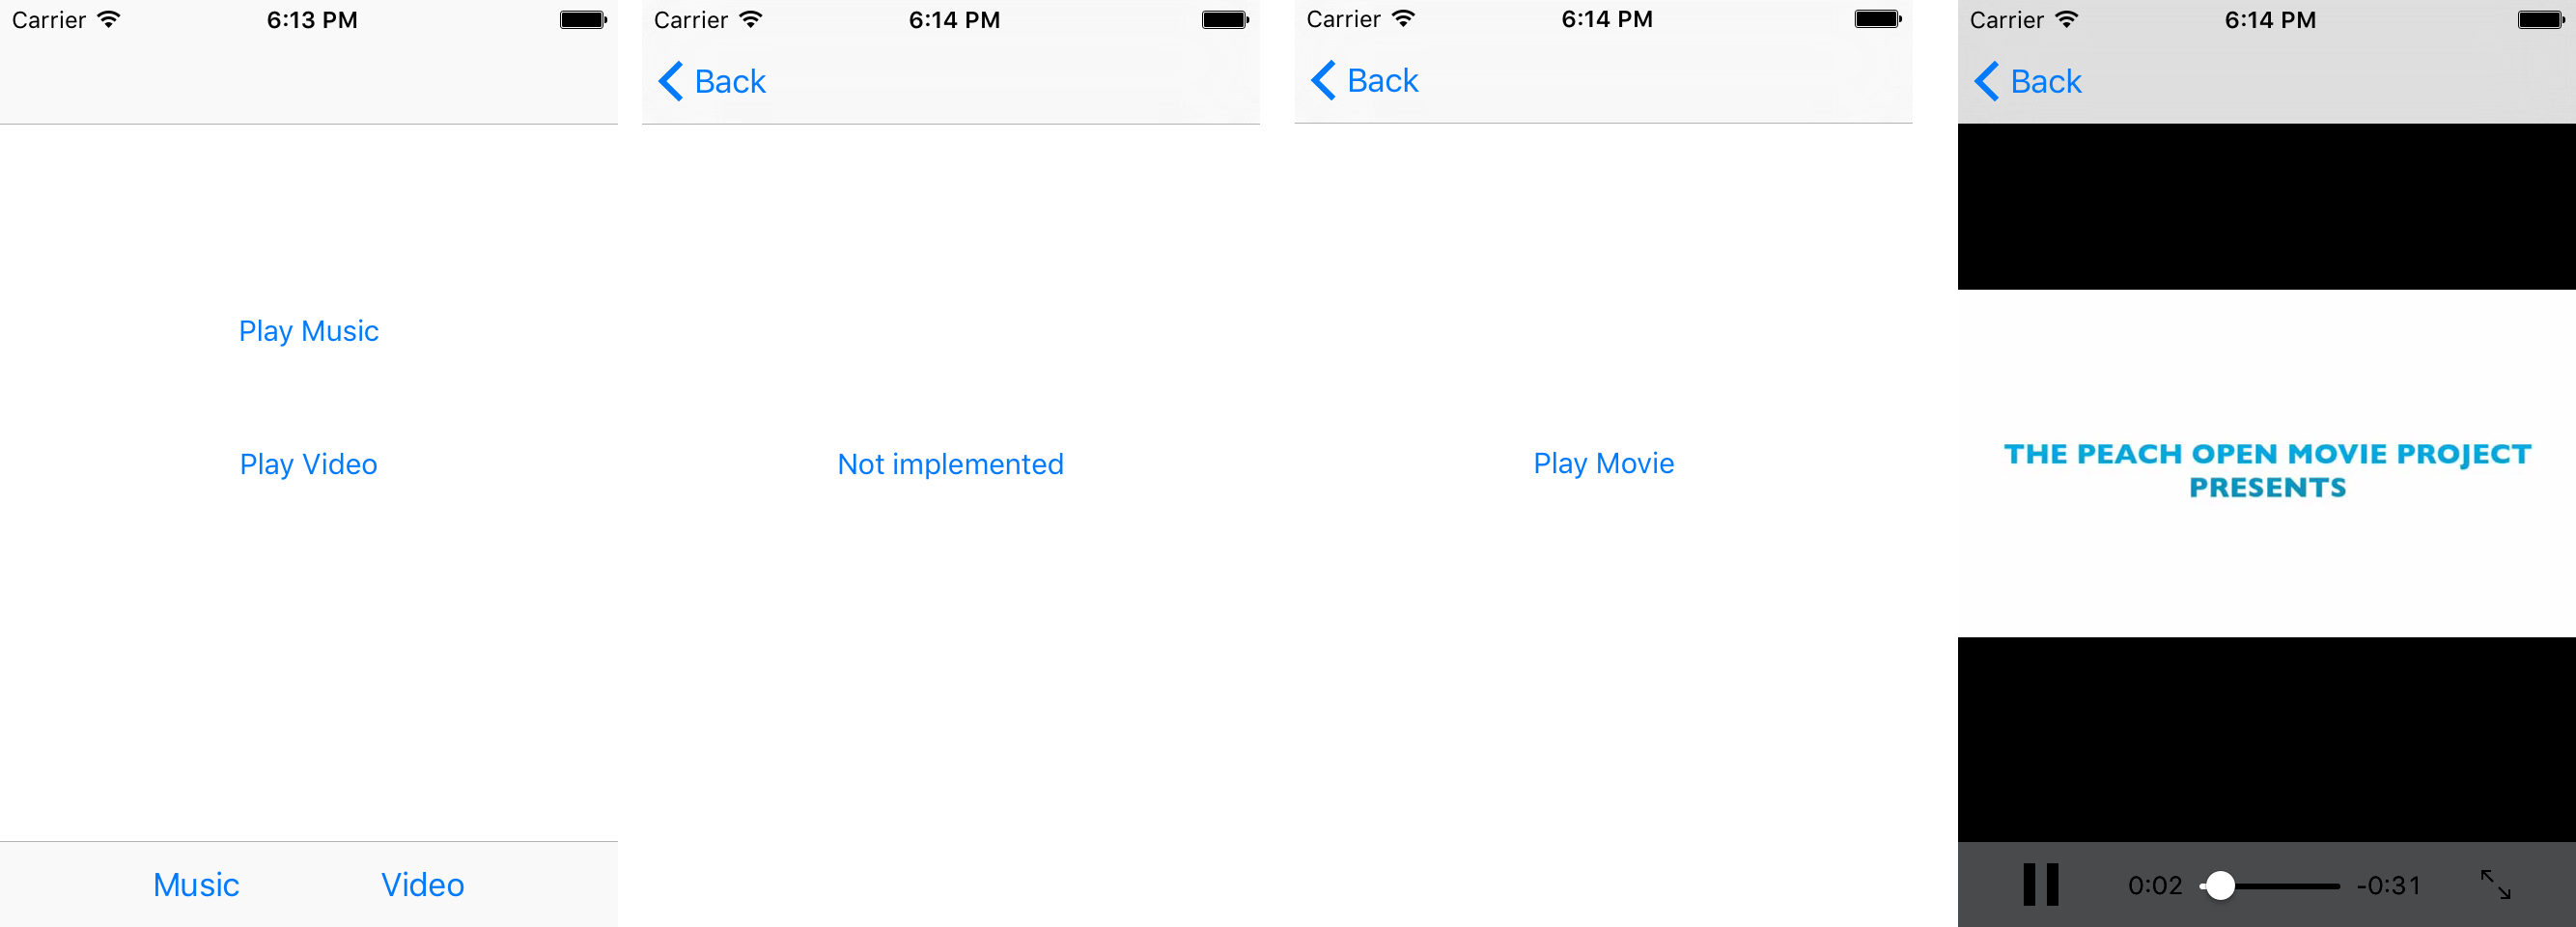
\includegraphics[width=16.5cm]{img/cas2_0.png}
		\caption{Vues de l'application réalisée}
		\label{vues3}
	\end{center}
\end{figure}
\textbf{Source de la vidéo:\\}
\url{http://jplayer.org/video/m4v/Big_Buck_Bunny_Trailer.m4v}\\

Le bouton Play Music, le Music de la toolbar ainsi qu'un swipe à droite ouvre la liste des musique. Cette vue n'étant pas implémentée, un simple message est affiché. \\
Le bouton Play Video, le Video de la toolbar ainsi qu'un swipe à gauche ouvre la vue pour lancer une vidéo.\\
Cette dernière contient un simple bouton qui va lancer la vidéo dans une autre vue. Le lecteur a été implémenté pour lire la vidéo en boucle. Le bouton stop et play fonctionnent correctement. Le bouton done par contre ne revient pas à la vue précédente, il stop simplement la lecture. Cette particularité est due au fait que le lecteur n'est pas implémenté directement dans la vue au bouton Play movie, mais dans une vue séparée.\\
Pour la navigation entre les vues, chacune possède un bouton back qui permet de retourner à la précédente.

